\documentclass{beamer}


\mode<presentation>
{
  \usetheme{CambridgeUS}
	\usecolortheme{beaver}
  % or ...

  \setbeamercovered{transparent}
  % or whatever (possibly just delete it)
}


\usepackage[absolute,overlay]{textpos}
\usepackage{subfig}

\usepackage{xeCJK}
\usepackage[english]{babel}
\usepackage[utf8]{inputenc}
\usepackage{times}
\usepackage[T1]{fontenc}
\usepackage{hyperref}
\usepackage{pifont}
\usepackage{biblatex}
\usepackage{bibentry}
\usepackage{verbatim}
\usepackage{ulem}
\bibliography{cite}
\newcommand{\cmark}{\ding{51}}%
\newcommand{\xmark}{\ding{55}}%
\setCJKmainfont{WenQuanYi Micro Hei}
\renewcommand{\raggedright}{\leftskip=0pt \rightskip=0pt plus 0cm}
\raggedright

\let\oldfootnotesize\footnotesize
\renewcommand*{\footnotesize}{\oldfootnotesize\tiny}

\title[Games and Software Engineering] 
{Games and Software Engineering}
\subtitle{Bug or Feature?}

\author[Zhilei Ren] 
{Zhilei Ren}

\institute[OSCAR Team] % (optional, but mostly needed)
{
\\
\includegraphics[width=0.2\textwidth]{../../utils/logo.jpg}\\
OSCAR Team, School of Software, 
Dalian University of Technology
}


\subject{Open Source}



\pgfdeclareimage[height=0.5cm]{university-logo}{../../utils/logo.jpg}
\logo{\pgfuseimage{university-logo}}



% Delete this, if you do not want the table of contents to pop up at
% the beginning of each subsection:
\AtBeginSubsection[]
{
  \begin{frame}<beamer>{Outline}
    \tableofcontents[currentsection,currentsubsection]
  \end{frame}
}


% If you wish to uncover everything in a step-wise fashion, uncomment
% the following command: 

%\beamerdefaultoverlayspecification{<+->}

\setbeamertemplate{section in toc}[circle]
\setbeamertemplate{items}[circle]
\setbeamertemplate{caption}[numbered]
\setbeamertemplate{bibliography item}{\insertbiblabel}
\setbeamertemplate{bibliography entry title}{}
\setbeamertemplate{bibliography entry journal}{}

\begin{document}

\begin{frame}
  \titlepage
\end{frame}

%\begin{frame}{Outline}
%  \tableofcontents[currentsection,currentsubsection, 
%    hideothersubsections, 
%    sectionstyle=show,
%]
%\end{frame}

\AtBeginSection[]
{
 \begin{frame}<beamer>
 \frametitle{Outline}
 \tableofcontents[currentsection]
 \end{frame}
}
\begin{frame}[t]{bug or feature?}
    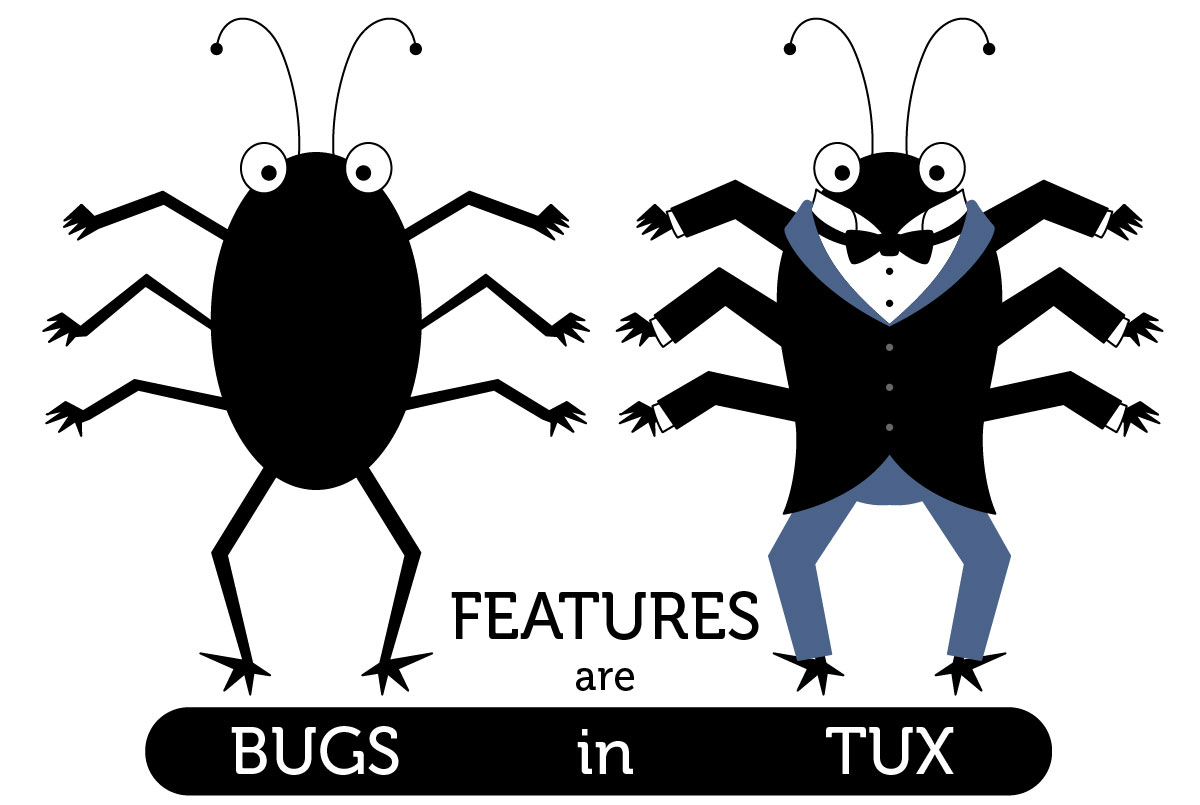
\includegraphics[width=.5\textwidth]{bugfeature.jpg}
\end{frame}
\begin{frame}[t]{第一个计算机bug}
    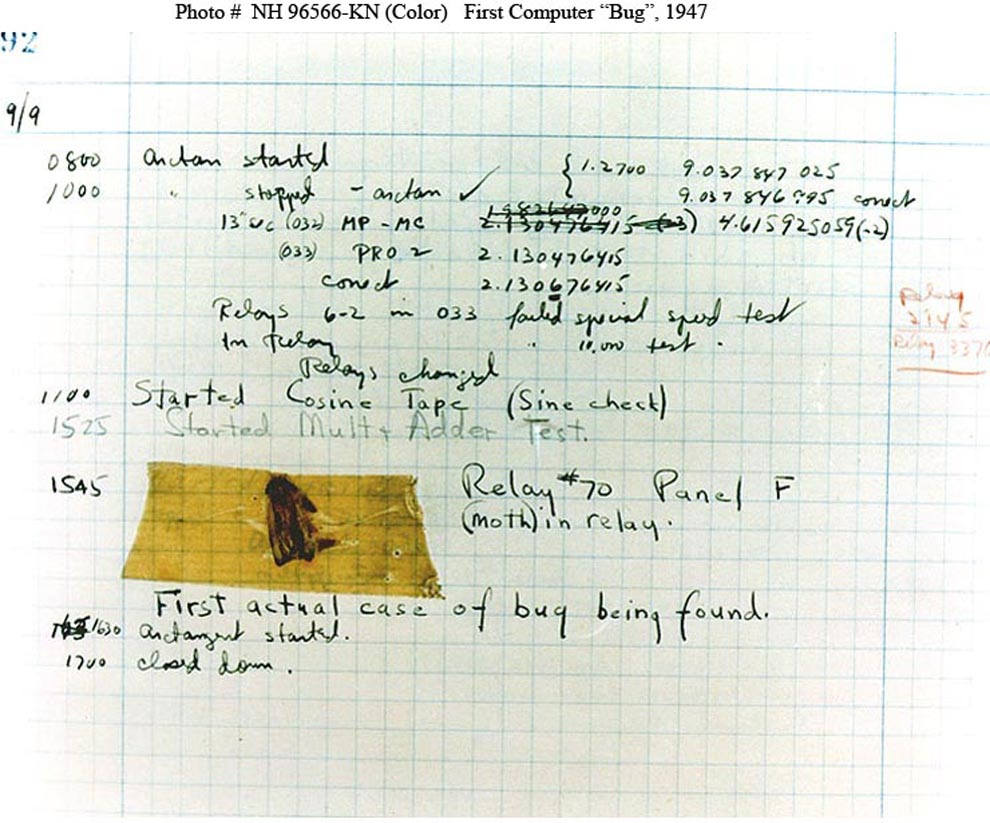
\includegraphics[width=.5\textwidth]{computer-bug.jpg}  
\end{frame}
\begin{frame}[t]{第一个计算机bug}
    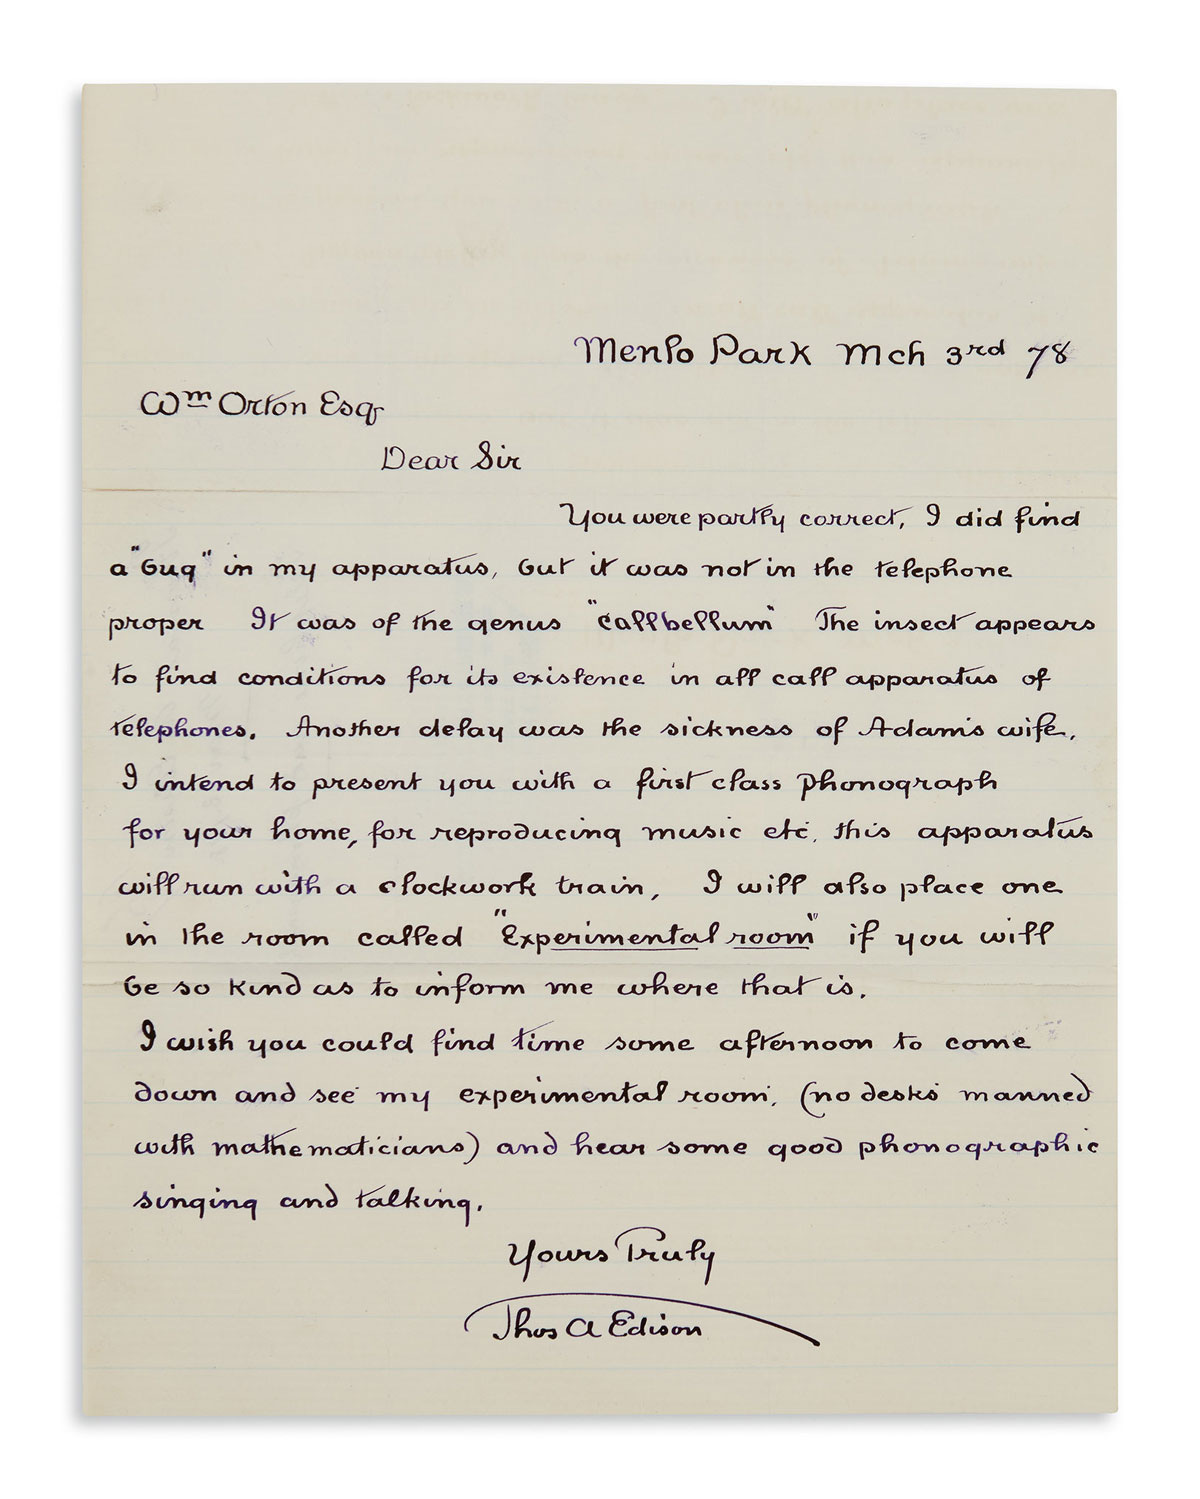
\includegraphics[width=.5\textwidth]{telebug.jpg}  
\end{frame}
\begin{frame}[t]{Combo}
    格斗对战游戏《街头霸王II》中采用了连招理念，掌握技巧的玩家可在恰当时间，连续击打电脑玩家，使之没有时间恢复及继续战斗。连招设计属于偶然；主制作人船水纪孝在程序查错时发现了这一情况，他虽然认为时机要求难度很大，难以当作游戏功能，但还是将之作为隐藏设定。此后连招成为格斗游戏的重要设计元素，方法从简单到高难度不一。《超级街头霸王II》是最早统计连击数，并奖励有达到连击的玩家的游戏。\footnote{\url{https://en.wikipedia.org/wiki/Combo_(video_games)}}        

    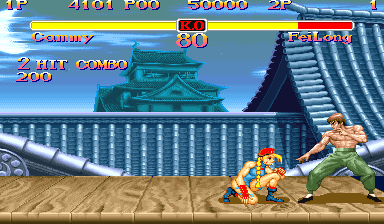
\includegraphics[width=.5\textwidth]{Super_Street_Fighter_II_screenshot.png}

\end{frame}


\begin{frame}[t]{Hidden Features aka Easter Egg}
    \begin{figure}
    \begin{center}
        
\includegraphics[width=.5\textwidth]{images/1280px-Konami_Code.svg.png}
    \end{center}
    \caption{Konami Code}
    \label{fig:konami}
    \end{figure}

    \pause
科乐美秘技起因是桥本和久手下一个人为了移植1985年射击游戏《宇宙巡航舰》（グラディウス）的商务用街机版到家庭红白机版时，而开发了投币式版本，但这个这个版本很难，桥本和久也并没有玩多久，并表示自己也打不过它，而又因为自己是要使用它的人并且为了确保指令很容易被大家记住，所以加入了科乐美秘技。原计划是移植完后删除，而后来因为秘籍浪潮而没删除\footnote{\url{https://en.wikipedia.org/wiki/Konami_Code}}. 
    \begin{textblock}{3}(12,3)
        \only<2>{
            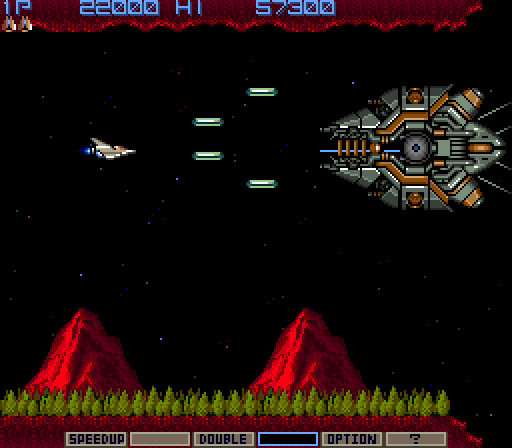
\includegraphics[width=\textwidth]{images/gradius.png}
        }
    \end{textblock}
\end{frame}

\begin{frame}[t]{慎用彩蛋}
        \begin{figure}[b]
        \centering
        \subfloat[Test Failure due to man]{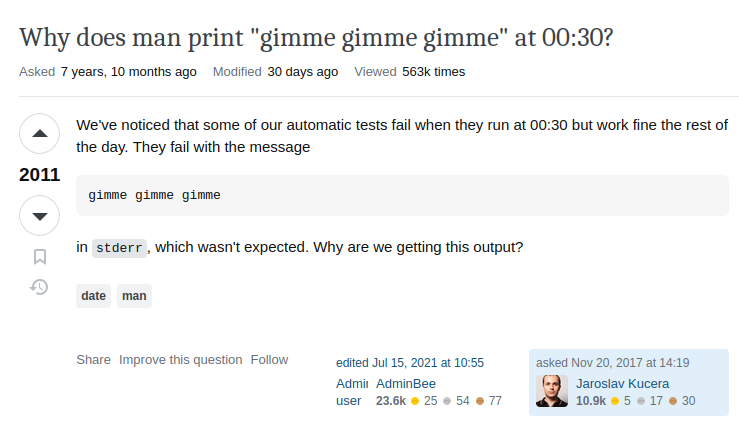
\includegraphics[width=5cm]{images/test_failure.png}}\qquad    
        \subfloat[The Root Cause]{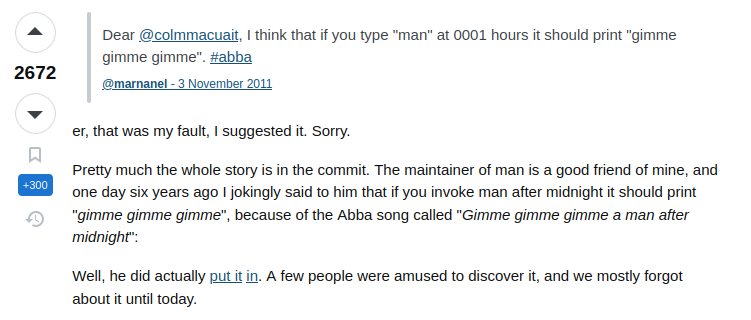
\includegraphics[width=5cm]{images/gimme.png}}    


        \caption{Bug Caused by an Easter Egg}
        \end{figure}
    
    
\end{frame}

\end{document}

